\documentclass[a4paper,12pt]{article}

\title{Exercise 5: Self Localization}
\author{Group 6:\\Niels\\Troels\\Mark\\Kristian}

\usepackage[T1]{fontenc}
\usepackage{lmodern}
\usepackage[utf8]{inputenc}
\usepackage[british]{babel}
\usepackage{microtype}
\usepackage{underscore}
\usepackage{amsmath}
\usepackage{graphicx}
\usepackage[hidelinks]{hyperref}

\setlength{\parskip}{1ex}
\setlength{\parindent}{0pt}
\setlength{\parfillskip}{30pt plus 1 fil}

\begin{document}

\maketitle

\section{Implementation}

\subsection{Particle Filter}
\begin{figure}[htp]
\centering
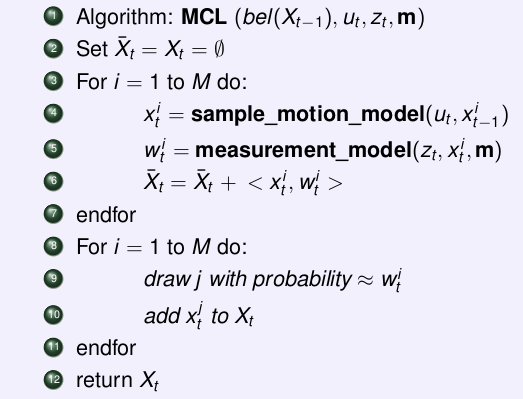
\includegraphics[scale=0.50]{MCL.png}
\caption{MCL lokalization algorithm}
\label{MCL}
\end{figure}

\subsection{Prediction step}
For the prediction step we use the function move\_particle in particle.cc. It corresponds with the sample\_motion\_model as in algorithm. \\
The move\_particle is fairly simple, It simply moves the particle position(x,y) with the given $\Delta x $ and $\Delta y$ if the control command were drive. If the robot turned we add $\Delta \theta$ to the particle $\theta$ value. \\
The given delta values are calculated with the robot speed and driving time. \\
$\Delta x = cos(p.\theta)\cdot\text{speed}\cdot 100$ \\
$\Delta y = sin(p.\theta)\cdot\text{speed}\cdot 100$ \\
After every prediction step we add some noise to the prediction with the function add\_uncertainty with parameters 5 cm and 5 degrees. 
\subsection{Calculating weights}
The weight of the particle can be calculated using hint 6 in the exercise. Thus the weight of the particle is the product: $p(d_M | x^{(i}, y^{(i)})) \cdot  p(\theta_M |x^{(i)} , y^{(i)} , \theta^{(i)} ) $. \\
The weights of the particle is calculated at landmark detection. The given code returns the distance and orientation to the landmark which we use the product. \\
The product consist of the gauss-distribution, so our implementation takes a difference and variance argument. The difference is either the difference between particle and landmark in dist or angle orientation. \\
After we calculated all the weights we normalize the particle weights by dividing with the total sum of weights. \\
\subsection{Resampling}
In order to resample we create a sum vector with consists of the cumulative sum of every particle weight which we use when we pick random an particle. By creating a cumulative sum vector we remove the possibility of particles with a weight of zero is getting picked.\\
When we pick particles we generate a random number z with randf().\\
Then we run through the sum vector until we get an entry which equal of greater than z. When this occurs we pick that particle with the given index. This is done num\_particles times, so we have consistent number of particles.\\
Each time we pick a particle we add it to a new vector which is set to be our working set of particles at the end of resampling.\\
This does unfortunately not work in practice of reasons we do not know. so created a more naive implementation: 
 

\subsection{Driving Strategy}




\end{document}
